\documentclass[a4paper]{article}

\usepackage[pdftex]{graphicx}
\usepackage[margin=3cm]{geometry}
\usepackage{verbatim,moreverb,amssymb,amsmath}


\newcounter{question}
\newcommand{\question}[1]{\refstepcounter{question}\section*{Question~\thequestion~~~\small\emph{(#1)}}}
\renewcommand*\thequestion{\arabic{question}}


\begin{document}

\pagestyle{empty}
\thispagestyle{empty}



\noindent
\begin{minipage}{\columnwidth}
  \centering
  \Large
  DA4002 (HT11) Halmstad University\\
  Introduction to Algorithms, Data Structures, and Problem Solving\\[3\baselineskip]
  \Huge
  Written Exam\\
  \Large
  Tuesday, October 30, 2012\\[2\baselineskip]
  Examiner: Roland Philippsen
\end{minipage}

\vfill

\noindent
\begin{center}
\fbox{
  \begin{minipage}{0.8\columnwidth}
    \textbf{Student Name:}\\[3\baselineskip]
  \end{minipage}
}
\end{center}

\vfill



\section*{Rules}

Aside from the obvious rules of conduct exams (e.g.\ no chatting):

\begin{itemize}
\item
  \textbf{No computing devices} (laptops, phones, calculators, \emph{etc}).
\item
  \textbf{No books or printouts} except for non-electronic dictionaries.
\item
  \textbf{Allowed hand-written notes}: two sheets of A4 paper (front and back).
\end{itemize}



\section*{General Guidelines}

\begin{itemize}
\item
  \textbf{Read carefully} and pace yourself.
  You can solve the problems in any order you want, but later problems may be easier to solve after you have answered the preceding questions.
\item
  \textbf{Write clearly} and draw clear diagrams.
  If you need to correct a mistake, then cleanly cross out the wrong answer and clearly indicate where the correction can be found.
\item
  \textbf{Indicate the question number} for each of your answers.
  If a question has sub-questions, indicate the sub-question number after the main question number, separated by a dot.
  For example, question 3 has 4 sub-questions, and their answers should be numbered 3.1, 3.2, 3.3, and 3.4.
\end{itemize}



\pagebreak
\pagestyle{plain}
\thispagestyle{plain}
\setcounter{page}{1}



\question{6 points}

Below are three diagrams \textbf{(1)}, \textbf{(2)}, and \textbf{(3)}.
Each of them shows the result of inserting the values $\{5, -2, -3, 1, 9, 6\}$ into a different type of data structure.
Beside the diagrams are three data structure declarations \textbf{(A)}, \textbf{(B)}, \textbf{(C)}.
Each of them corresponds to one of the diagrams.
On the next page, there are three different implementations of an \textbf{\texttt{insert}} function.
They are labelled \textbf{(D)}, \textbf{(E)}, \textbf{(F)}.
Each implementation is for a different type of data structure.

\begin{enumerate}
\item
  Fill in the table at the bottom of this page.
  For each of the diagrams
  \begin{itemize}
  \item
    choose the corresponding declaration (from this page),
  \item
    choose the corresponding implementation (from the next page),
  \item
    and write down the name of the data structure.
  \end{itemize}
\item
  For each of these data structures, write code that iterates over all the items and prints their value.
  You can use pseudo-code or C code, or plain English.
\end{enumerate}

\vfill

\noindent
\begin{minipage}{0.4\columnwidth}
  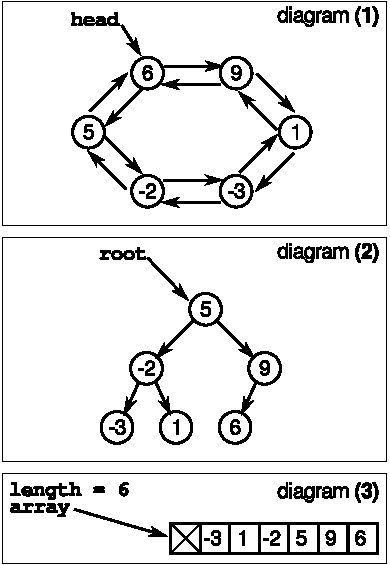
\includegraphics[width=\columnwidth]{q1.pdf}
\end{minipage}\hfill
\begin{minipage}{0.5\columnwidth}
  \small
  \fbox{%
    \begin{minipage}{\columnwidth}
      \hfill declaration \textbf{(A)}
      \verbatimtabinput{clist-decl.txt}
  \end{minipage}}
  \fbox{%
    \begin{minipage}{\columnwidth}
      \hfill declaration \textbf{(B)}
      \verbatimtabinput{minheap-decl.txt}
  \end{minipage}}
  \fbox{%
    \begin{minipage}{\columnwidth}
      \hfill declaration \textbf{(C)}
      \verbatimtabinput{bstree-decl.txt}
  \end{minipage}}
\end{minipage}

\vfill

\begin{center}
  \begin{tabular}{|c|p{0.2\columnwidth}|p{0.2\columnwidth}|p{0.5\columnwidth}|}
    \hline
            & declaration  & implementation & \\
    diagram & (A, B, or C) & (D, E, or F)   & data structure name \\
    \hline
    &&&\\
    \textbf{(1)} & & & \\
    &&&\\
    \hline
    &&&\\
    \textbf{(2)} & & & \\
    &&&\\
    \hline
    &&&\\
    \textbf{(3)} & & & \\
    &&&\\
    \hline
  \end{tabular}
\end{center}


\clearpage

\subsection*{Implementations for Question 1}

\noindent
\fbox{%
  \begin{minipage}{\columnwidth}
    \hfill implementation \textbf{(D)}
    \footnotesize
    \verbatimtabinput{minheap-insert.txt}
\end{minipage}}

\noindent
\fbox{%
  \begin{minipage}{\columnwidth}
    \hfill implementation \textbf{(E)}
    \footnotesize
    \verbatimtabinput{bstree-insert.txt}
\end{minipage}}

\noindent
\fbox{%
  \begin{minipage}{\columnwidth}
    \hfill implementation \textbf{(F)}
    \footnotesize
    \verbatimtabinput{clist-insert.txt}
\end{minipage}}


\clearpage

\question{4 points}

In a \emph{multilist}, items have multiple link fields and belong to independently maintained linked lists.
For example, we can store planar points sorted along the X and the Y coordinate at the same time.
The two linked lists rely on two link fields, in this case one for the next item along X, and one for the next item along Y.
We also need to maintain two separate heads, because the start of the list that is sorted along X will usually be different from the start of the list that is sorted along Y.

The diagram shows five planar points labeled \textbf{A}, \textbf{B}, \textbf{C}, \textbf{D}, and \textbf{E}, each with different X and Y coordinates.
Below that is a sketch of a \emph{multilist} which should be used to store these points such that:

\begin{itemize}
\item
  We can traverse the list of points by order of increasing X coordinate by starting at \texttt{xhead} and repeatedly following the \texttt{xnext} link.
\item
  And for visiting the points in order of increasing Y coordinate, we start at \texttt{yhead} and follow the \texttt{ynext} links.
\end{itemize}

\vfill

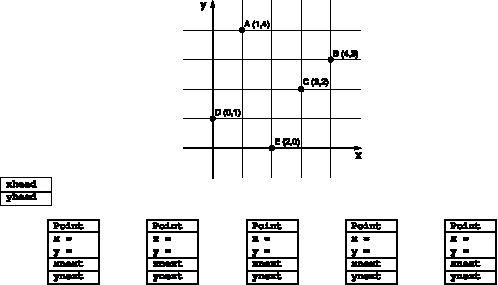
\includegraphics[width=\columnwidth]{q2.pdf}

\vfill

\begin{enumerate}
\item
  For each of the \texttt{Point} boxes above, fill in the point label (A, B, C, D, E) and the coordinates, then draw arrows from the \texttt{xnext} fields to an appropriate \texttt{Point} box, such that the resulting linked list is sorted along X (from lowest to highest) and contains all the points A, B, C, D, and E.
  Don't forget to draw an arrow from the \texttt{xhead} box.
  Then, do the same for the Y coordinate, on top of the same diagram.
\item
  Write down the procedure to insert a point, given by its X and Y coordinates, into such a multilist.
  You have to provide a declaration for the data structure that you are using, and don't forget to handle the case when the list is empty.
\end{enumerate}

\clearpage

\question{4 points}




\clearpage

\question{6 points}


\clearpage

\question{5 points}



\end{document}
